\documentclass[a4paper, 12pt]{article}
\usepackage[english]{babel}
\usepackage[utf8]{inputenc}
\usepackage[T1]{fontenc}
\usepackage{lmodern}

\usepackage{url}
\usepackage{graphicx}

\usepackage{amsmath}
\usepackage{amsthm}
\usepackage{amsfonts}


\theoremstyle{definition}
\newtheorem{definicija}{Definicija}

\theoremstyle{plain}
\newtheorem{izrek}{Izrek}

% ne spreminjaj podatkov, ki vplivajo na obliko strani
\textwidth 15cm
\textheight 24cm
\oddsidemargin.5cm
\evensidemargin.5cm
\topmargin-5mm
\addtolength{\footskip}{10pt}
\pagestyle{plain}
\overfullrule=15pt % oznaci predlogo vrstico


% ukazi za matematicna okolja


% za stevilske mnozice uporabi naslednje simbole
\newcommand{\R}{\mathbb R}
\newcommand{\N}{\mathbb N}
\newcommand{\Z}{\mathbb Z}
\newcommand{\C}{\mathbb C}
\newcommand{\Q}{\mathbb Q}
\newcommand{\f}{\mathcal F}
\newcommand{\p}{\mathbb P}

% ukaz za slovarsko geslo
\newlength{\odstavek}
\setlength{\odstavek}{\parindent}


% naslednje ukaze ustrezno popravi
\newcommand{\program}{Finančna matematika} % ime studijskega programa: Matematika/Finan'cna matematika
\newcommand{\imeavtorja}{Tia Krofel, Brina Ribič, Matej Rojec} % ime avtorja
\newcommand{\imementorja}{dr. Aleš Ahčan} % akademski naziv in ime mentorja
\newcommand{\naslovdela}{VaR on option portfolio}
\newcommand{\letnica}{2022}


\begin{document}

% od tod do povzetka ne spreminjaj nicesar
\thispagestyle{empty}
\noindent{\large
UNIVERZA V LJUBLJANI\\[1mm]
FAKULTETA ZA MATEMATIKO IN FIZIKO\\[5mm]
\program\ -- 2.~stopnja}
\vfill

\begin{center}{\large
\imeavtorja\\[2mm]
{\bf \naslovdela}\\[10mm]
Seminarska naloga pri predmetu Upravljanje tveganj\\[1cm]
Mentor: \imementorja}
\end{center}
\vfill

\noindent{\large
Ljubljana, \letnica}
\pagebreak

\thispagestyle{empty}
\tableofcontents
\pagebreak

\section{Osnovno o opcijah}

Opcija je pogodba med nosilcem opcije (kupcem) in izdajateljem opcije
o nakupu oziroma prodaji osnovnega premoženja (temelja) po določeni ceni $K$ imenovani
izvršilna cena. Če opcija daje nosilcu pravico nakupa temelja, jo imenujemo nakupna opcija, če pa daje pravico prodaje,
jo imenujemo prodajna opcija. Glede na to, kdaj je možna izvršitev opcije, ločimo več vrst opcij.
Najbolj preprosta je evropska opcija, ki daje pravico izvršitve samo ob zapadlosti. Ameriška opcija
daje pravico izvršitve kadarkoli do vključno trenutka zapadlosti. Poznamo tudi druge vrste opcij, ki jih skupno imenujemo eksotične opcije.

Označimo s $t=0$ čas izadje opcije, s $t=T$ pa čas zapadlosti.
Naj bo $S_t$ cena osnovnega premoženja ob času $t\in [0,T]$.
Vrednost opcije za nosilca opcije je enaka razliki med ceno osnovnega premoženja v času
izvršitve in izvršilno ceno, če je zanj pozitivna. Sicer opcije ne izvrši in je njena
vrednost enaka $0$. Izplačilo evropske nakupne opcije ob času T je
\begin{equation}
    C_T = max\{S_T-K,0\},
\end{equation}
saj se mu v primeru, ko je $S_T<K$ ne splača izvršiti opcije, torej je njeno izplačilo $0$.
Izplačilo evropske prodajne opcije pa je enako 
\begin{equation}
    P_T = max\{0, K-S_T\}.
\end{equation}

Kupec opcije mora ob nakupu opcije plačati premijo. Kako visoka je ta premija, je precej komplicirano izračunati.
Premijo oziroma vrednost opcije bomo računali z Black-Scholesovim modelom. Cena evropske prodajne opcije ob času $t$ je 
\begin{equation}\label{prodajna}
    V_t = Ke^{-R(T-t)}\Phi(-d_2)-S_t\Phi(-d_1),
\end{equation}
kjer je
\begin{itemize}
    \item $K$ izvršilna cena opcije,
    \item $R$ netvegana obrestna mera,
    \item $S_0$ cena temelja ob času $0$.
\end{itemize}
Konstanti $d_1$ in $d_2$ izračunamo s formulama
\begin{equation}
    \begin{aligned}
        d_1 &= \frac{\ln(\frac{S_0}{K}e^{RT})+\frac{\sigma^2}{2}T}{\sigma\sqrt{T}},\\
    d_2 &= d_1-\sigma\sqrt{T}. 
    \end{aligned}
\end{equation}
Tu je $\sigma$ volatilnost donosov temelja. Podobno formulo dobimo za izračun premije evropske nakupne opcije
\begin{equation}\label{nakupna}
    V_t = S_t\Phi(d_1) - Ke^{-R(T-t)}\Phi(d_2).
\end{equation}

Glavna predpostavka v tem modelu je, da ima temelj zvezno neodvisno enako normalno porazdeljene donose.
Naš cilj bo oceniti tveganje opcij glede na temelj. To bomo naredili s t. i. grškimi parametri.

%While the type (put or call) and the underlying stock are self-evident and essentially standardized, the striking price and expiration date require more
%explanation. 

%Striking prices intervals are not hardcoded, they are detirmened on an exchange.
%They are generally spaced 5 points apart, but for expensive stock they and be 
%10 points or more apart andfFor cheaper stocks (i.e. less then \$35 per share)
%they can be 2.5 points apart. However these intervals can be altered, based on 
%market depth and liqudity.

% B-S model
% grki
% zaščitni portfelj

\section{Osnovno o VaR}

"Value at Risk" oziroma VaR je mera, ki je opredeljena kot največja potencialna sprememba v vrednosti portfelja pri določeni,
dovolj visoki stopnji zaupanja za vnaprej določeno časovno obdobje. Ponavadi je stopnja zaupanja $95\%$ ali $99\%$.
VaR nam pove, koliko lahko izgubim z $x\%$ verjetnostjo v nekem časovnem obdobju. Ponavadi se uporablja
krajše časovno obdobje, recimo dan, teden ali nekaj tednov.
To pomeni, če je VaR za neko sredstvo $100$ milijonov evrov v obdobju enega tedna s stopnjo zaupanja $95\%$,
potem je samo $5\%$ verjetnost, da bo vrednost sredstva padla za več kot $100$ milijonov evrov v katerem koli tednu.

Let us now give a formal definiton of value at risk. 
\begin{definicija}
Let $X$ be a random variable on a probability space $(\Omega, \f, \p)$ and $\alpha \in (0, 1)$.
VaR$_\alpha(X)$ is defined as the $(1-\alpha)$ quntile of -$X$. So:
$$
\textnormal{VaR}_\alpha(X) := - \inf \{ x \in \R \mid F_X(x) > \alpha \} = F^{-1}_{-X}(1-\alpha).
$$
\end{definicija}

Obstajajo trije osnovni pristopi, kako izračunati VaR. Lahko ga izračunamo analitično
s predpostavkami o porazdelitvah donosov za tržna tveganja, zraven pa moramo upoštevati variance
in kovariance med temi tveganji. VaR lahko ocenimo tudi s hipotetičnim portfeljem preko historičnih 
podatkov ali z Monte Carlo simulacijo. 

Nas bo zanimalo, kaj se zgodi, če imamo sredstvo, ki je izvedeni finančni instrument. V tem primeru moramo 
nekoliko modificirati VaR.
Recimo pri opcijah, moramo pri oceni tveganja upoštevati nelinarno gibanje cen (gamma učinek)
in posredna volatilnost (vega učinek). % implied volatilities
Za opcije bomo nelinearno gibanje cen ocenili analitično (delta-gamma) ali s simulacijo.


\subsection{Kako izračunamo VaR}

\subsubsection{Variančno-kovariančna metoda}

Variančno-kovariančna metoda je parametrična metoda, ki predpostavlja, da so donosi, 
kateri določajo vrednost portfelja,
porazdeljeni normalno. Slučajna spremenljivka je porazdeljena normalno s parametroma $\mu$ (povprečje)
in varianco $\sigma^2$ oziroma standardnim odklonom $\sigma$, če je gostota podana z 
\begin{equation}
    f(x) = \frac{1}{\sigma\sqrt{2\pi}}exp[-\frac{1}{2}(\frac{x-\mu}{\sigma})^2],
\end{equation}
kjer je $x\in \R$. Ta metoda je uporabna, ker je v celoti definirana samo z dvema parametroma. 
Hkrati nam zagotavlja direktne formule za izračun kumulativnih porazdelitvenih funkcij; velja namreč
\begin{equation}
    P(X<x) = \mu + \alpha_{cl}\sigma,
\end{equation}
kjer je $cl$ izbrana stopnja zaupanja (npr. $95\%$) in $\alpha_{cl}$ je standardna normalna spremenljivka pri izbrani stopnji zaupanja
(npr. $\alpha_{0.95}=1.645$). 

VaR za eno naložbo je potem enak
\begin{equation}
    VaR = MV\cdot \alpha_{cl} \cdot \sigma,
\end{equation}
kjer je $MV$ tržna vrednost temelja. Pri izračunu VaR za portfelj, ki je sestavljen iz več pozicij,
moramo upoštevati tudi diverzifikacije oziroma razpršitve naložb.
% dodaj še natančnejši opis
Pri opcijah se ta metoda izkaže za učinkovito, potrebno jo je le nekoliko modificirati. Ker je vrednost opcije odvisna od več dejavnikov 
ter imamo nelinearno povezavo med vrednostjo opcije in donosnostjo temelja, moramo izračunati še nekaj dodatnih parametrov, da bo rezultat korekten.

\subsubsection{Zgodovinska simulacija}
Zgodovinska simulacija omogoča zelo preprosto in intuitivno oceno VaR. Temelji na vrstnem redu opazovanih podatkov;
recimo, da imamo $100$ opažanj, potem je šesto po vrsti VaR pri stopnji zaupanja $95\%$. 
Zavedati pa se moramo, da lahko pride do večjih napak pri tem načinu izračuna VaR zaradi ekstremnih dogodkov, dolžine opazovanega obdobja, \dots
Prav tako ta metoda ni primerna za izračun nelinernega VaR oziroma 
za izračun VaR za opcije, saj je historične podatke za opcije težko dobiti in jih med seboj primerjati.

\subsubsection{Monte Carlo simulacija}
Monte Carlo simulacija je danes v praksi zelo uporabna saj je precej prilagodljiva za veliko različic VaR. 
Izkazalo se bo, da je uporabna tudi za izračun nelinearnega VaR.

\section{Nelinearen VaR}

Osnovna različica VaR predpostavlja linearno povezavo med donosi in spremembo vrednosti pozicije
oziroma da je relativna sprememba portfelja linearna funkcija donosa temelja (delnice, obveznice \dots)
Tu predpostavljamo, da imajo donosi vrednostnega papirja večrazsežno normalno porazdelitev.  

Vrednost pozicij pri izvedenih finančnih instrumentih je odvisna od vrednosti od nekega drugega vrednostnega papirja.
Pri opcijskih pozicijah je nelinearna povezava med spremembo vrednosti pozicije in donosom temelja. 
To lahko pojasnimo s preprosto opcijo na delnico. Cena opcije je $V(S_t,K,T,R,\sigma)$ v 
odvisnosti od cene delnice $S_t$ ob času $t$, izvršilne cene $K$, časa dospelosti $T$. 
Cena opcije je odvisna tudi od netvegane obrestne mere $R$ nekega vrednostnega papirja, ki ima enak
čas dospelosti kot opcija ter od standardnega odklona $\sigma$ cene temelja v časovnem obdobju opcije. 
Zato moramo uporabiti drugačen pristop za računanje VaR za portfelj iz opcij. 

\begin{figure}\label{payoff}
    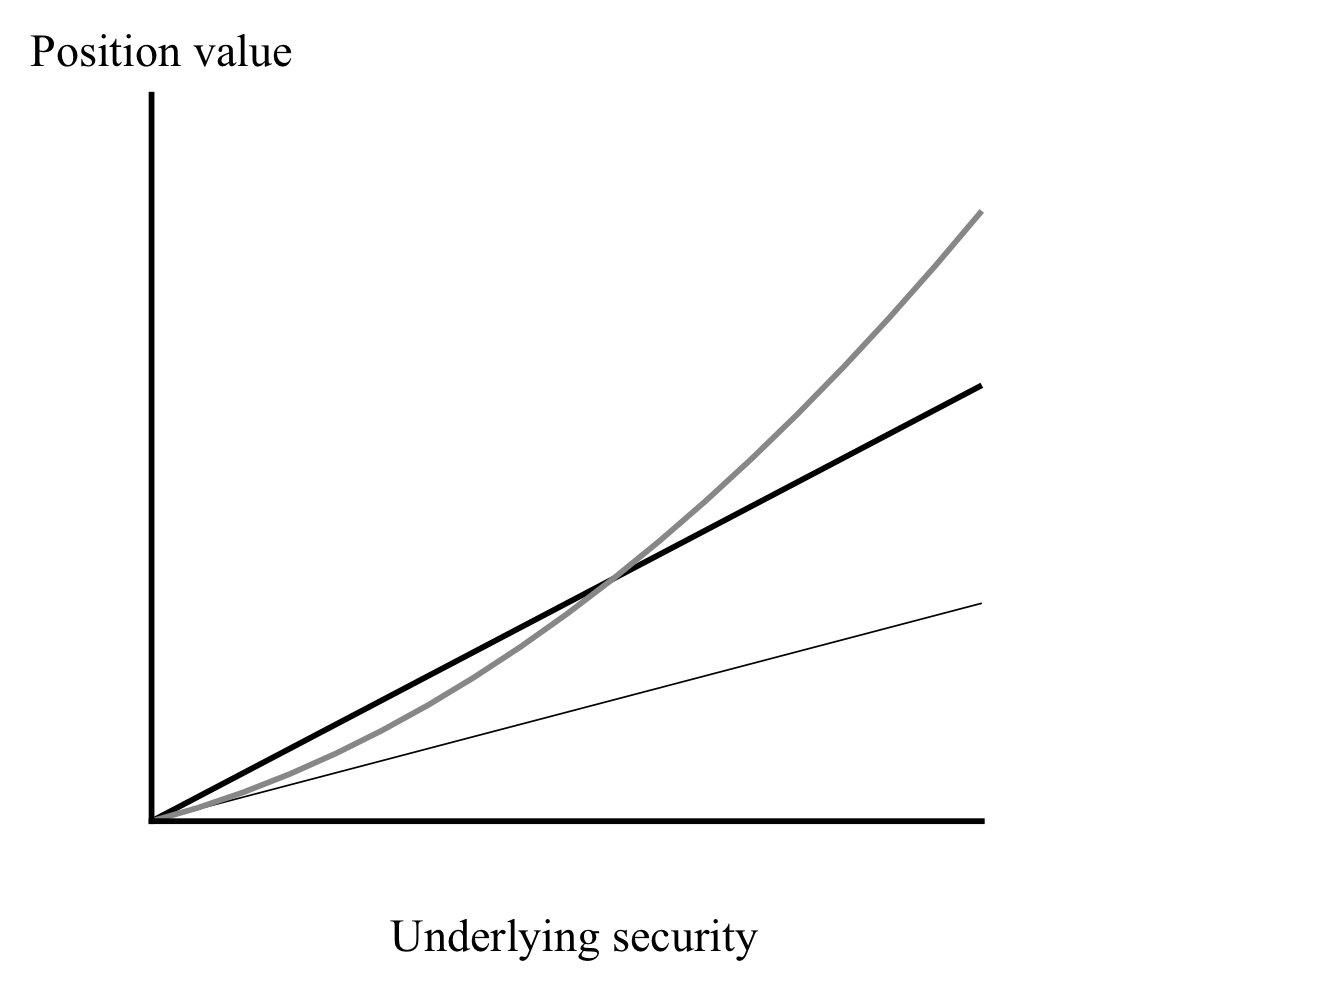
\includegraphics[width=0.7\textwidth]{payoff.jpg}
    \caption{Linearna in nelinearna funkcija izplačila.}
\end{figure}

Na sliki \ref{payoff} je prikazana vrednost pozicije glede na temelj. 
Ravni črti predstavljata linearno zvezo med vrednostjo pozicije in vrednostjo temelja. 
Vrednost evropske opcije (nakupne ali prodaje) bomo izrazili z "delta". To pomeni, da zveza
med vrednostjo pozicije in vrednostjo temelja ne bo več linearna ampak nelinearna. Na grafu to 
predstavlja siv graf funkcije. Opazimo, da ni več linearna funkcija.
V primeru, ko je zveza linearna, je "delta" $-1$ ali $1$. Če pa je "delta" katero koli drugo število
med $-1$ in $1$, govorimo o nelinearni povezavi med vrednostjo pozicije in vrednostjo temelja.
Dodatno potrebujemo parameter "gamma", s katerim bomo definirali konveksnost funkcije. Pri linearnih zvezah
je "gamma" vedno enak $0$ in imajo konstanten naklon. Pri nelinearnih zvezah, recimo pri opcijah, pa je 
"gamma" vedno neničelno nenegativno število. Od tod izhajajo različni pristopi za računanje nelinearnega VaR.


Pri vseh različicah še vedno predpostavljamo, da so donosi vrednostnih papirjev porazdeljeni normalno. 
Dodatno dopuščamo nelinearno zvezo med vrednostjo pozicije in donosi temelja. Natančneje, dovoljujemo gama učinek,
torej da relativna sprememba portfelja iz derivativov (v našem primeru opcij) ni več normalno porazdelja. 
Zaradi tega ne moremo več VaR definirati kot 1.65 krat standardni odklon portfelja. Namesto tega VaR 
izračunamo v dveh glavnih korakih. Najprej izračunamo prve štiri momente porazdelitve donosa portfelja, tj.,
povprečje, standardni odklon, \textbf{skewness}, \textbf{kurtosis}. Potem poiščemo 
porazdelitev, ki ima enake prve štiri momente kot porazdelitev donosa portfelja in izračunamo peti 
percentil (ali prvi, odvidno od problema). Od tod dobimo VaR.




\end{document}